

\chapter{The OpenRocket simulation software}
\label{chap-software}

The flight simulation described in the previous chapters was
implemented in the {\it OpenRocket} simulation
software~\cite{openrocket}.  The software was written entirely in Java
for maximum portability between different operating systems.  A
significant amount of effort was put into making the graphical user
interface (UI) robust, intuitive and easy to use.  As of the first
public release the source code contained over 300 classes and over
47\s000 lines of code (including comments and blank lines).

The software was released under the copyleft GNU General Public
License (GPL)~\cite{gnu-gpl}, allowing everybody access to the source code
and permitting use and modification for any purposes.  The only major
restriction placed is that if a modified version is distributed, the
source code for the modifications must also be available under the GNU
GPL.  This ensures that the program stays free and Open Source; a
company cannot simply take the code, enhance it and start selling it
as their own without contributing anything back to the community.

In this section the basic architectural designs are discussed and the
main features of the UI are explained.



\section{Architectural design}

The software has been split into various components within their own
Java packages.  This enables use of the components without needing the
other components.  For example, all of the UI code is within the
\code{gui} package, and the simulation system can be used
independently of it.


The rocket structure is composed of components, each with their
own class defined within the package \code{rocketcomponent}.  This
provides the base for defining a rocket.  The components are described
in more detail in Section~\ref{sec-rocket-components}.  The simulation
code is separated from the aerodynamic calculation code in the
\code{simulation} and \code{aerodynamics} packages, respectively;
these are discussed in Section~\ref{sec-simulator-calculator}.

The package naming convention recommended in the Java Language
Specification is followed~\cite{java-packages}.  Therefore all package
names discussed herein are relative to the package
\url{info.openrocket}.  For example, the rocket components are
defined in the package \url{info.openrocket.core.rocketcomponent}.




\subsection{Rocket components}
\label{sec-rocket-components}

The structure of the rocket is split up into {\it components}, for
example nose cones, body tubes and components within the rocket body.
Each component type is defined as a subclass of the abstract
\code{RocketComponent} class.  Each component can contain zero or more
components attached to it, which creates a tree structure containing
the entire rocket design.  The base component of every design is a
\code{Rocket} object, which holds one or more \code{Stage} objects.
These represent the stages of the rocket and hold all of the physical
components.

Inheritance has been highly used in the class hierarchy of the
components in order to combine common features of various components.
There are also some abstract classes, such as \code{BodyComponent},
whose sole purpose currently is to allow future extensions.  The
complete component class hierarchy is presented as a UML diagram in
Figure~\ref{fig-rocketcomponent-uml}, and a more detailed description
of each class is presented in Table~\ref{table-rocketcomponents}.

\begin{sidewaysfigure}
\centering
\hspace{-1cm}
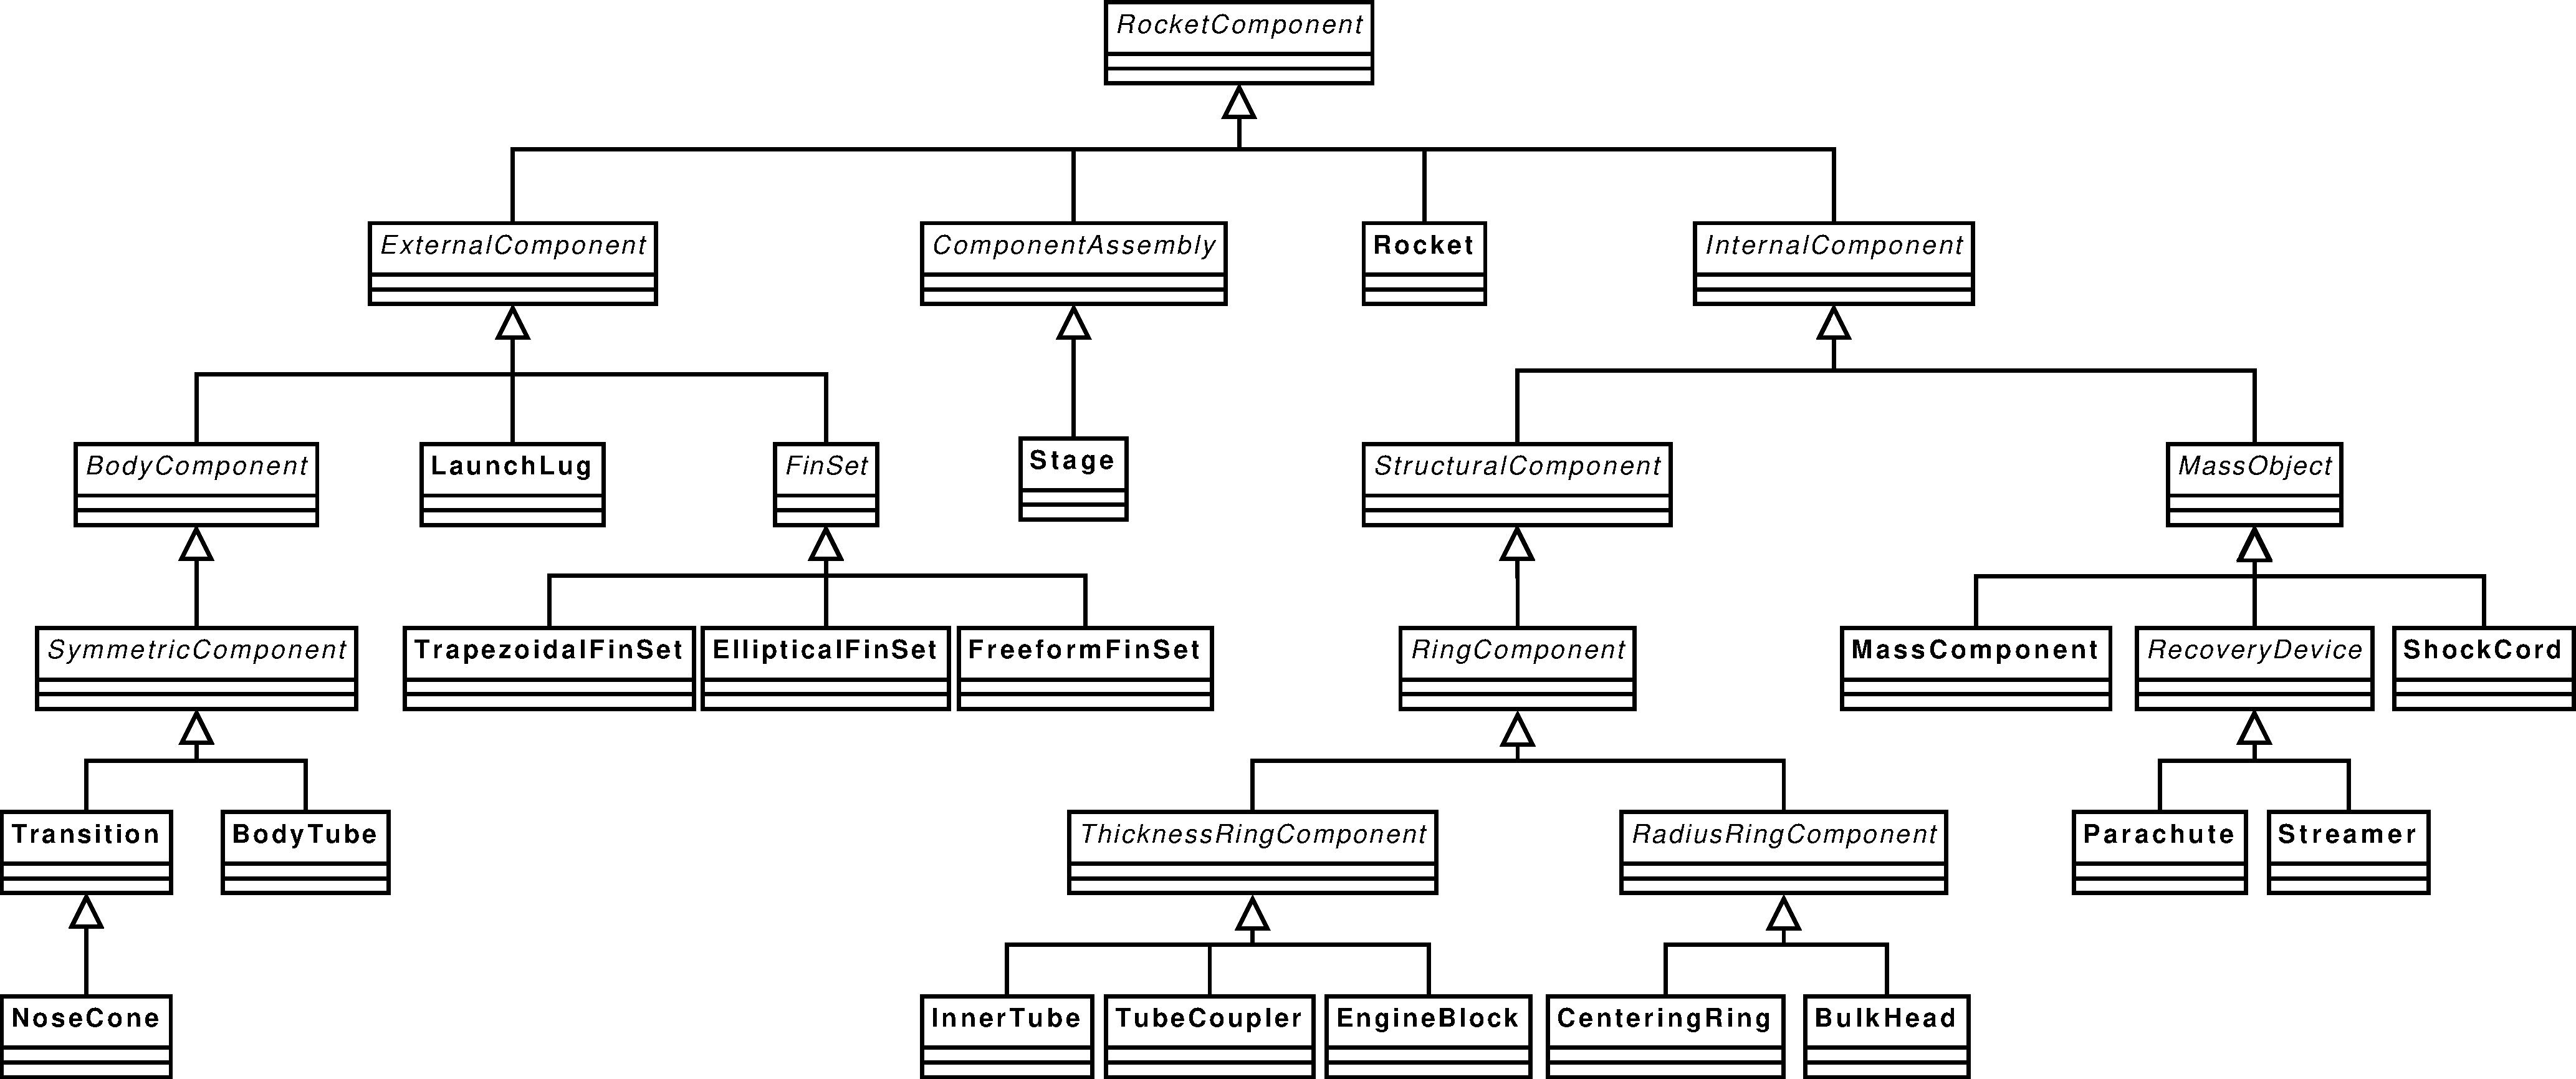
\epsfig{file=figures/software/rocketcomponents,width=20cm}
\caption{A UML diagram of the rocket component classes.  Abstract
  classes are shown in italics.}
\label{fig-rocketcomponent-uml}
\end{sidewaysfigure}


\begin{table}
\caption{Descriptions of the rocket component classes and their
  functionality.  Abstract classes are shown in italics.}
\label{table-rocketcomponents}
\sloppy\footnotesize
\vspace{\baselineskip}
\hspace{-5mm}\begin{tabular}{lp{80mm}}
Component class & Description \\
\hline
\code{\textit{RocketComponent}}: &
  The base class of all components,
  including common features such as child component handling. \\

\hspace{3mm}\code{Rocket}: &
  The base component of a
  rocket design, provides change event notifications. \\

\hspace{3mm}\code{\textit{ComponentAssembly}}: &
  A base component for an assembly of external components.  This could
  in the future be extended to allow multiple rocket bodies next to
  each other. \\

\hspace{6mm}\code{Stage}: &
  A separable stage of the rocket. \\

\hspace{3mm}\code{\textit{ExternalComponent}}: &
  An external component that has an effect on the aerodynamics of the
  rocket. \\

\hspace{6mm}\code{\textit{BodyComponent}}: &
  A portion of the main rocket body, defined in cylindrical coordinates
  by $r = f(x, \theta)$. \\

\hspace{9mm}\code{\textit{SymmetricComponent}}: &
  An axisymmetrical body component. \\

\hspace{12mm}\code{Transition}: &
  A symmetrical transition (shoulder or boattail). \\

\hspace{15mm}\code{NoseCone}: &
  A transition with the initial radius zero. \\

\hspace{12mm}\code{BodyTube}: &
  A cylindrical body tube.  Can be used as a motor mount. \\

\hspace{6mm}\code{\textit{FinSet}}: &
  A set of one or more fins. \\

\hspace{9mm}\code{TrapezoidalFinSet}: &
  A set of trapezoidal fins. \\

\hspace{9mm}\code{EllipticalFinSet}: &
  A set of elliptical fins. \\

\hspace{9mm}\code{FreeformFinSet}: &
  A set of free-form fins. \\

\hspace{6mm}\code{LaunchLug}: &
  A launch lug or rail pin. \\

\hspace{3mm}\code{\textit{InternalComponent}}: &
  An internal component that may affect the mass of the rocket but not
  its aerodynamics. \\

\hspace{6mm}\code{\textit{StructuralComponent}}: &
  A structural internal component, with specific shape and density. \\

\hspace{9mm}\code{\textit{RingComponent}}: &
  A hollow cylindrical component. \\

\hspace{12mm}\code{\textit{ThicknessRingComponent}}: &
  A component defined by an outer radius and shell thickness. \\

\hspace{15mm}\code{InnerTube}: &
  An inner tube.  Can be used as a motor mount and can be clustered. \\

\hspace{15mm}\code{TubeCoupler}: &
  A coupler tube. \\

\hspace{15mm}\code{EngineBlock}: &
  An engine block. \\

\hspace{12mm}\code{\textit{RadiusRingComponent}}: &
  A component defined by an inner and outer radius. \\

\hspace{15mm}\code{CenteringRing}: &
  A ring for centering components. \\

\hspace{15mm}\code{Bulkhead}: &
  A solid bulkhead (inner radius zero). \\

\hspace{6mm}\code{\textit{MassObject}}: &
  An internal component shaped approximately like a solid cylinder and
  with a specific mass. \\

\hspace{9mm}\code{MassComponent}: &
  A generic component with specific mass, for example payload. \\

\hspace{9mm}\code{\textit{RecoveryDevice}}: &
  A recovery device. \\

\hspace{12mm}\code{Parachute}: &
  A parachute. \\

\hspace{12mm}\code{Streamer}: &
  A streamer. \\

\hspace{9mm}\code{ShockCord}: &
  A shock cord with a specified material and length. \\

\hline
\end{tabular}
\end{table}


Additionally four interfaces are defined for the components,
\code{MotorMount}, \code{Clusterable}, \code{Radial\-Parent} and
\code{Coaxial}.  Components implementing the \code{Motor\-Mount}
interface, currently \code{Body\-Tube} and \code{Inner\-Tube}, can
function as motor mounts and have motors loaded in them.  The
\code{Clusterable} interface signifies that the component can be
clustered in various configurations.  Currently only the
\code{Inner\-Tube} component can be clustered.  Components and motors
that are attached to a clustered inner tube are automatically
replicated to all tubes within the cluster.  The \code{Radial\-Parent}
interface allows inner components to automatically identify their
correct inner and outer radii based on their parent and sibling
components.  For example, a coupler tube can automatically detect its
radius based on the inner radius of the parent body tube.
\code{Coaxial} on the other hand provides a generic interface for
accessing and modifying properties of fixed-radius components. 


Since the software functionality is divided into different packages,
all component similarities cannot be directly be exploited through
inheritance.  For example, the method of drawing a nose cone shape
belongs to the \url{gui.rocketfigure} package, however, it can share
the same code that draws a transition.  For these purposes, reflective
programming is used extensively.  The code for drawing both nose cones
and transitions is provided in the class
\code{gui.rocketfigure.SymmetricComponentShapes}, while the simpler
body tube is drawn by the class \code{BodyTubeShapes}.  The correct
class is derived and instantiated dynamically based on the component
class.  This allows easily sharing functionality common to different
components while still having loose coupling between the rocket
structure, presentation, computation and storage methods.




\subsection{Aerodynamic calculators and simulators}
\label{sec-simulator-calculator}

One of the key aspects in the design of the simulation implementation
was extensibility.  Therefore all aerodynamic calculation code is
separated in the package \code{aerodynamics} and all simulation code
is in the package \code{simulator}.  This allows adding new
implementations of the aerodynamic calculators and simulators
independently.  For example, a simulator using Euler integration was
written in the early stages of development, and later replaced by the
Runge-Kutta~4 simulator.  Similarly, a different method of calculating
the aerodynamic forces, such as CFD, could be implemented and used by
the existing simulators.

The basis for all aerodynamic calculations is the interface
\code{Aerodynamic\-Calculator}.  The current implementation, based on
the Barrowman methods, is implemented in the class
\code{Barrowman\-Calculator}.  This implementation caches mid-results
for performance reasons.

Flight simulation is split into the
interfaces \code{Simulation\-Engine}, which is responsible for
maintaining the flow of the simulation and handling events (such as
motor ignition), and \code{Simulation\-Stepper}, which is responsible
for taking individual time steps while simulating (using {\it e.g.}
RK4 iteration).

Similar abstraction has been performed for the atmospheric temperature
and pressure model with the \code{Atmospheric\-Model} interface, the
gravity model with \code{Gravity\-Model}, the wind modelling with
\code{Wind\-Model} and different rocket motor types by the
\code{Motor} class, among others.





\subsection{Simulation listeners}
\label{sec-listeners}

Simulation listeners are pieces of code that can dynamically be
configured to listen to and interact with a simulation while it is
running.  The listeners are called before and after each simulation
step, each simulation event and any calculations performed during
flight simulation.  The listeners may simply gather flight data for
use outside the simulation or modify the rocket or simulation during
the flight.  This allows great potential for extensibility both
internally and externally.

Listeners are used internally for various purposes such as retrieving
flight progress information when the user is running simulations and
cancelling the simulations when necessary.  Implementing such
functionality otherwise would have required a lot of special case
handling directly within the simulation code.

Listeners can also be used to modify the simulation or the rocket
during its flight.  The successor project of Haisun��t� included
an active roll stabilization system, where a flight computer 
measured the roll rate using two magnetometers and used a PID controller
to adjust two auxiliary fins to cancel out any roll produced by
inevitable imperfections in the main fins.  A simulation listener was
written that initially simulated the PID controller purely in Java, which
modified the cant angle of the auxiliary fins during the simulation.
Later a similar listener interfaced the external flight computer
directly using a serial data link.  The listener fed the simulated
flight data to the controller which computed and reported the control
actions back to the simulator.  This system helped identify and fix
numerous bugs in the flight computer software, which would have
otherwise been nearly impossible to fully test.  It is expected that
the simulation listeners will be an invaluable tool for more ambitious
model rocket enthusiasts.

A listener is produced by implementing the \code{Simulation\-Listener}
and optionally \code{Simulation\-Event\-Listener} and
\code{Simulation\-Computation\-Listener} interfaces, or by extending
the \code{Abstract\-Simulation\-Listener} class.  The UI includes the
option of defining custom simulation listeners to be utilized during
flight simulation.


\subsection{Warnings}
\label{sec-warnings}

The aerodynamic calculations and simulations are based on certain
assumptions and simplifications, such as a low angle of attack and a
smooth, continuous rocket body.  The rocket component architecture
makes it possible to create designs that break these assumptions.
Instead of limiting the options of the design, the aerodynamic
calculator and simulator can produce warnings about such issues.
These warnings are presented to the user during the design of the
rocket or after simulations.  It is then left up to the user to judge
whether such violations are significant enough to cast doubt to the
validity of the results.


\subsection{File format}

An XML-based file format was devised for storing the rocket designs
and simulations.  The use of XML allows using many existing tools for
reading and writing the files, allows easy extensibility and makes the
files human-readable.  The user has the option of including all
simulated data in the file, storing the data at specific time
intervals or storing only the simulation launch conditions.  To reduce
the file size, the files can additionally be compressed using the
standard GZIP compression algorithm~\cite{GZIP}.  The files are
compressed and uncompressed automatically by the software.  The file
extension .ORK was chosen for the design files, an abbreviation of the
software name that at the same time had no previous uses as a file
extension.





\section{User interface design}

The user interface was designed with the intent of being robust but
yet easy to use even for inexperienced users.  The main window,
depicted in Figure~\ref{fig-main-window}(a) with the design of the
original Haisun��t� rocket, consists of a schematic drawing of the
rocket, the tree structure of the rocket components and
buttons for adding new components to the structure. Components can
be selected or edited by clicking and double-clicking either the tree
view or the component in the schematic diagram.  The selected
components are drawn in bold to give a visual clue to the position
of the component.

The schematic drawing can be viewed either from the side or from the
rear, can be zoomed in and out and rotated along the centerline.  The
schematic diagram view also presents basic information about the
rocket, such as the design name, length, maximum diameter, mass and
possible warnings about the design. It also calculates the CG and CP
positions continuously during design and shows them both numerically
and on the diagram.  Additionally, a simulation is automatically run
in the background after each modification and the main results are
presented in the lower left corner of the diagram.  Many users are
interested in the maximum altitude or velocity of the rocket, and this
allows an immediate feedback on the effect of the changes they are
making to the design.  The flight information typically takes less
than a second to update.

The upper part of the main window can also be changed to view
simulation results, Figure~\ref{fig-main-window}(b).  Many simulations
can be added with different launch conditions and motor configurations
to investigate their effects.  Each simulation has a row which
presents the basic information about the simulation.  The first column
gives an immediate visual clue to the status of the simulation; a gray
ball indicates that the simulation has not been run yet, green
indicates an up-to-date simulation, red indicates that the design has
been changed after the simulation was run and yellow indicates that
the simulation information was loaded from a file, but that the file
states it to be up-to-date.  The simulations can be run one or several
at a time.  The software automatically utilizes several threads when
running multiple simulations on a multi-CPU computer to utilize the
full processing capacity.

Figure~\ref{fig-various-dialogs} shows two dialogs that are used
to modify and analyze the designs.  The components are edited using a
small dialog window that allows the user to either fill in the exact
numerical values specifying the shape of the component or use sliders
to modify them.  The user can change the units by clicking on them, or
set default values from the preferences.  Different tabs allow control
over the mass and CG override settings, figure color options, motor
mount and cluster options and more.  The Component analysis dialog
shown in the figure can be used to analyze the effect of individual
components on the total stability, drag and roll characteristics of
the rocket.

Similarly, the launch conditions and simulator options can be edited
in the corresponding dialog.  The simulator options also allow the
user to define custom simulation listeners to use during the
simulations.  The simulation edit dialog is also used for later data
analysis.  The simulated data can be plotted in a variety of ways as
shown in Figure~\ref{fig-plotting}.  The user can use predefined plot
settings or define their own.  Up to 15 different variables out of the
47 quantities computed can be plotted at a time.  The variable on the
horizontal axis can be freely selected, and the other variables can be
plotted on one of two vertical axis, on either side of the plot.  The
user can either specify whether a variable should plot on the left or
right axis or let the software decide the most suitable axis.  Typical
plots include the altitude, vertical velocity and acceleration of the
rocket with time or the drag coefficient as a function of the Mach
number.


\begin{figure}
\hspace{-7mm}
\begin{tabular}{m{1mm}m{10cm}}
\hspace{-5mm}(a) &
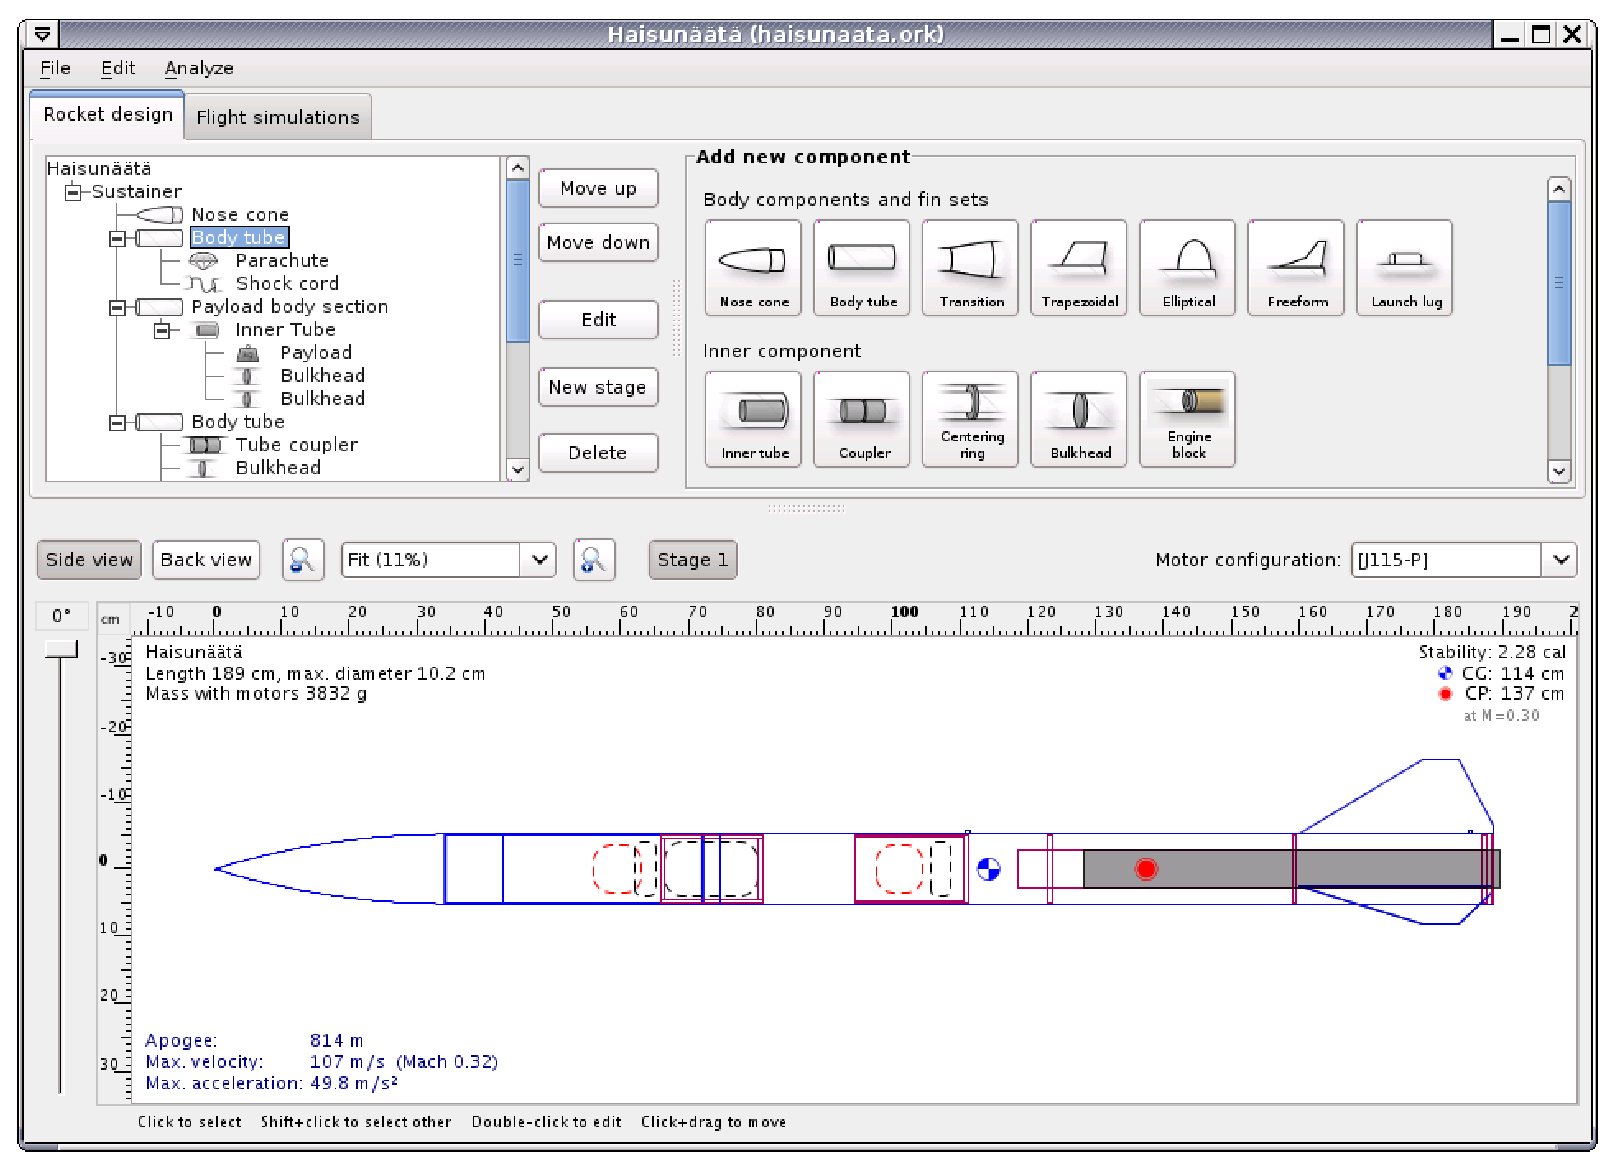
\epsfig{file=figures/pix/openrocket-main-haisunaata,scale=0.5} \\
\hspace{-5mm}(b) &
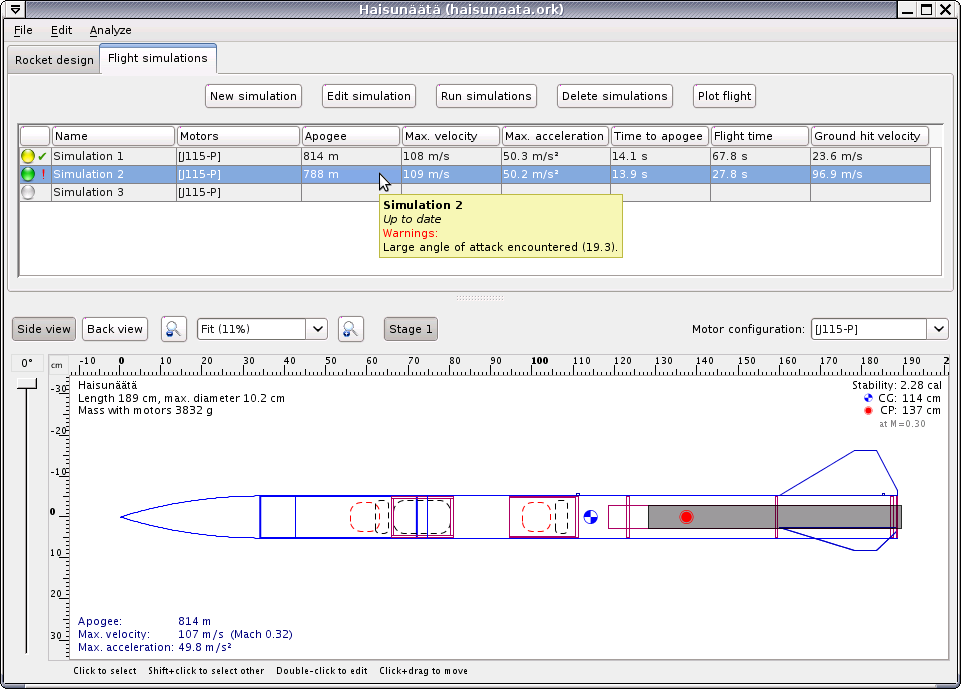
\epsfig{file=figures/pix/openrocket-simulations-haisunaata,scale=0.5}

\end{tabular}
\caption{The main design window of OpenRocket; (a) the design
  view and (b) the simulation view.}
\label{fig-main-window}
\end{figure}

\begin{figure}
\centering
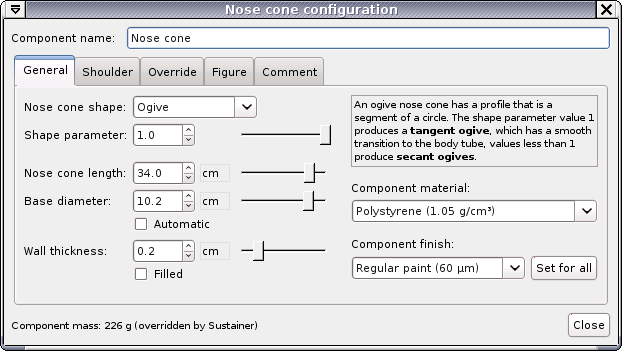
\epsfig{file=figures/pix/openrocket-dialog-edit,scale=0.5}
\vspace{2cm} \\
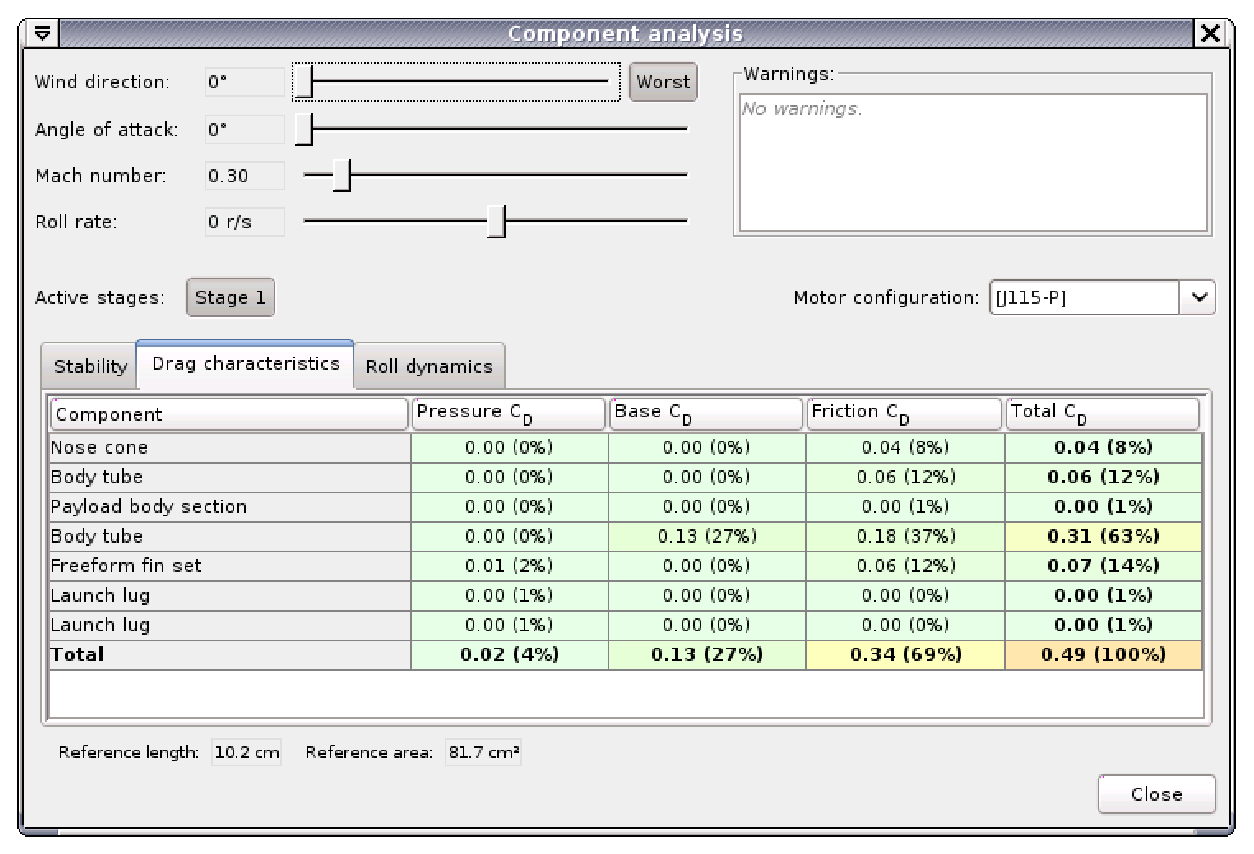
\epsfig{file=figures/pix/openrocket-dialog-analysis,scale=0.5}
\vspace{1cm} \\
\caption{Dialog windows for editing the properties of a nose cone
  and for analyzing the influence of individual components on
  the stability, drag and roll characteristics of the rocket.}
\label{fig-various-dialogs}
\end{figure}

\begin{figure}
\centering
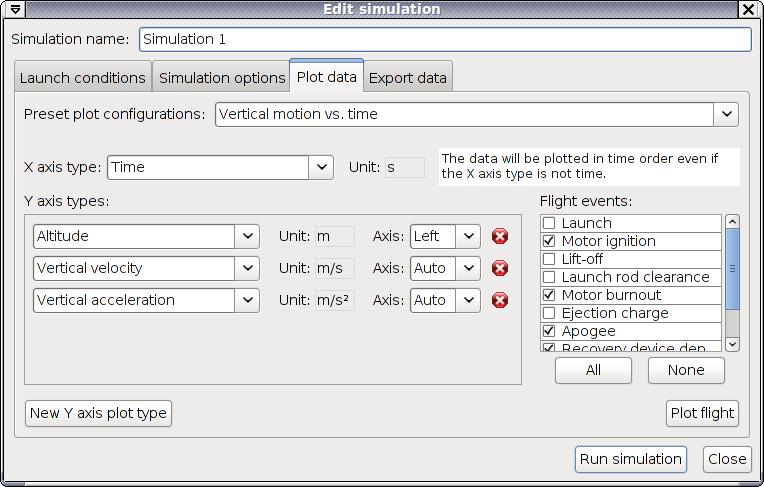
\epsfig{file=figures/pix/openrocket-dialog-plot-options,scale=0.5}
\vspace{2cm} \\
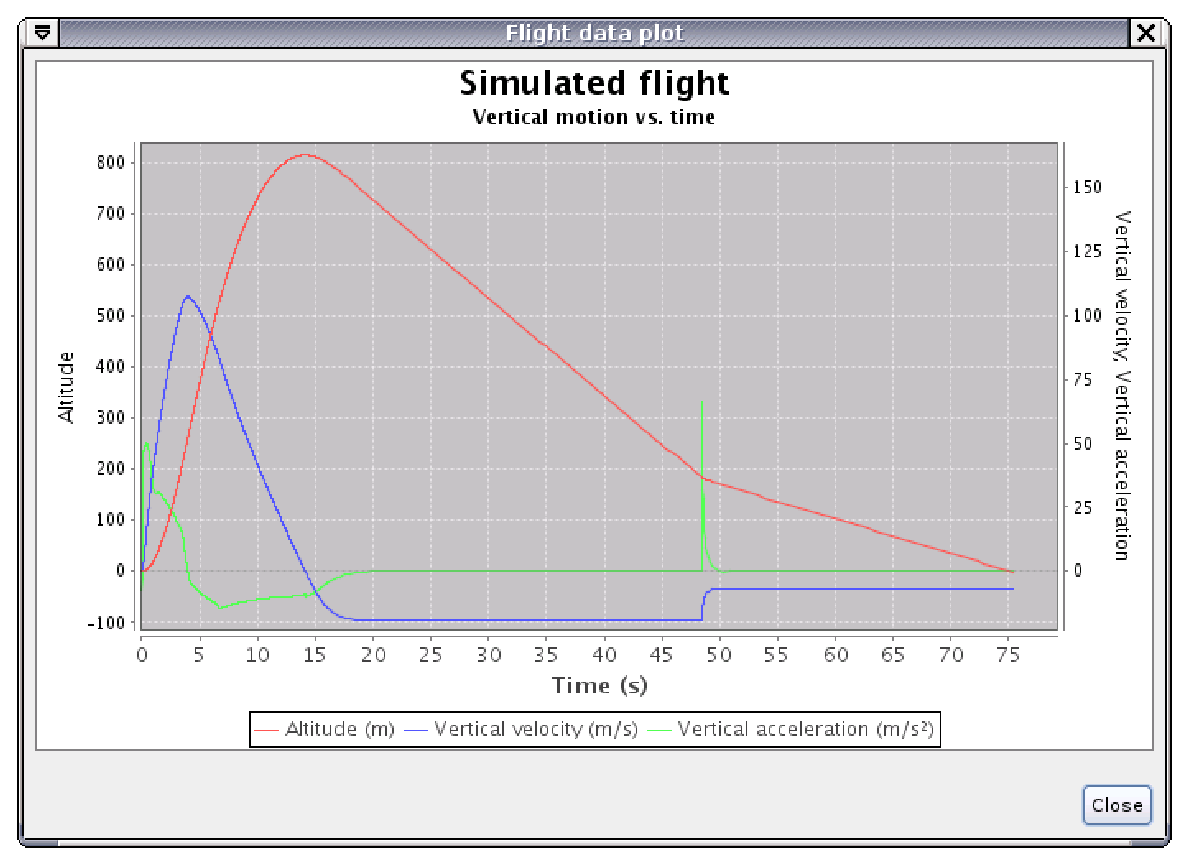
\epsfig{file=figures/pix/openrocket-dialog-plot,scale=0.5}
\vspace{1cm} \\
\caption{Dialog window for changing the simulation plot options and a
  plot of the simulated flight of the Haisun��t� hybrid rocket.}
\label{fig-plotting}
\end{figure}

Advanced users may also export the flight data in CSV format for
further analysis using other tools.

%
%\section{Future enhancements}
%
%Numerous features have been planned and taken into account during the
%design of the software.  Below are listed a few of the planned
%features and how they have been taken into account:
%
%{\it Alternative aerodynamic calculators.}  For example CFD could be
%used to calculate the aerodynamic properties, allowing even better
%simulation accuracy.  The calculators have been abstracted by the
%\code{AerodynamicCalculator} interface so they can easily be
%interchanged.
%
%{\it Alternative simulators.}  These could take into account for
%example the curvature of the Earth and include the Coriolis effect.
%New simulators can be created by implementing the
%\code{Simulation\-Stepper} interface.
%
%{\it Export and import of flight data.}  The simulated data could be
%exported for further analysis as comma separated values (CSV).
%Similarly, experimental data could be imported either from files or
%directly from altimeters.  Support for imported data already exists in
%the core functionalities.
%
%{\it Importing database files.}  The motor database is easily
%extendable to read external thrust curves.  Also data of commercially
%available rocket components could be imported and available in the
%component edit dialog.
%
%{\it Further UI enhancements.}  These could include for example a 3D
%view of the rocket, an animation of the rocket flight, a ``wizard''
%dialog for easily creating new designs, {\it etc.}
%
